\chapter{Исследовательская часть}

В данном разделе приведены технические характеристики устройства, на котором проводилось измерение времени работы программного обеспечения, а также результаты замеров времени.

\section{Технические характеристики}

Технические характеристики устройства, на котором выполнялись замеры по времени представлены далее.

\begin{itemize}[label=---]
	\item Процессор: Intel(R) Core(TM) i5-10300H CPU 2.50 ГГц~\cite{intel}.
	\item Количество ядер: 4 физических и 8 логических ядер.
	\item Оперативная память: 16 ГБайт.
	\item Операционная система: Windows 11 Pro 64-разрядная система~\cite{windows}.
\end{itemize}

При замерах времени ноутбук был включен в сеть электропитания и был нагружен только системными приложениями.

\section{Демонстрация работы программы}

На рисунке~\ref{img:example} представлен пример результата работы программы. 
Пользователь, указывая соответствующие пункты меню, запускает последовательную обработку заявок, затем параллельное исполнение конвейера, затем выходит из программы. Лог программы при этом на экран не выводится — он записывается в файл. 
На рисунке~\ref{img:log} представлен пример лог–файла.

\begin{figure}[h]
	\centering
	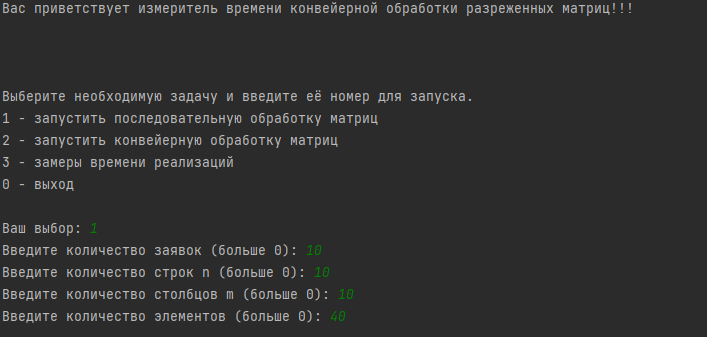
\includegraphics[width=0.85\textwidth]{img/example.png}
	\caption{Пример работы программы}
	\label{img:example}
\end{figure}

\begin{figure}[h]
	\centering
	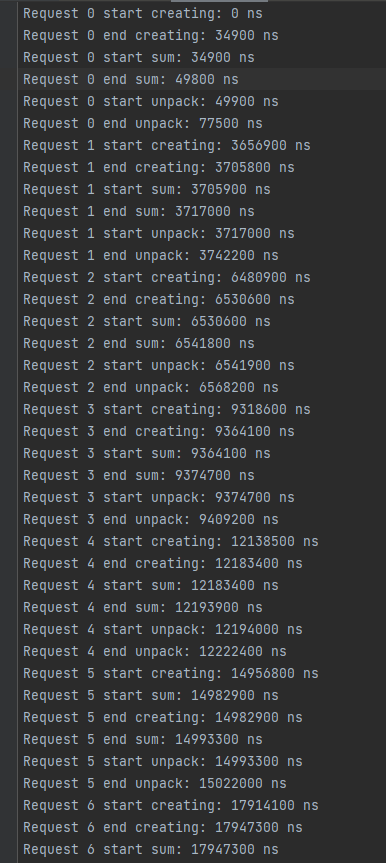
\includegraphics[height=0.5\textheight]{img/log.png}
	\caption{Пример файла с логом работы конвейера}
	\label{img:log}
\end{figure}

\clearpage

\section{Временные характеристики}

Для замеров времени использовалась функция получения значения системных часов $clock\_gettime()$~\cite{cpp-time}. Функция применялась два раза --- в начале и в конце измерения времени, значения полученных временных меток вычитались друг из друга для получения времени выполнения программы.
Замеры проводились по 100 раз для набора заявок от 10 до 100 штук с шагом 10. 

В таблице  \ref{tbl:time} представлены замеры времени выполнения двух реализаций конвейерной обработки в зависимости от количества заявок.

\begin{table}[ht]
	\small
	\begin{center}
		\begin{threeparttable}
		\caption{Результаты нагрузочного тестирования (в мкс)}
		\label{tbl:time}
		\begin{tabular}{|c|c|c|}
			\hline
			\multirow{2}{*}{\bfseries Кол-во заявок} & \multicolumn{2}{c|}{\bfseries Время, мкс} \\ \cline{2-3}
			 & \bfseries Последовательный & \bfseries Параллельный
			\csvreader{csv/times.csv}{}
			{\\\hline \csvcoli & \csvcolii & \csvcoliii } \\
			\hline
		\end{tabular}
		\end{threeparttable}
	\end{center}
\end{table}

На рисунке~\ref{img:g1} приведен график результатов замеров для различных значений количества.

\clearpage

\begin{figure}[h!]
	\centering
	\begin{tikzpicture}
		\begin{axis}[	
			height = 0.4\paperheight, 
			width = 0.8\paperwidth,
			legend pos = north west,
			table/col sep=comma,
			xlabel={кол-во заявок (ед.)},
			ylabel={время, мкс},
			]
			\legend{ 
				Последовательный,
				Параллельный,
			};
			\addplot [
			solid,
			thick, 
			draw = blue,
			mark = --, 
			mark options = {
				scale = 2, 
				fill = blue, 
				draw = black
			}
			] table [x=size, y=l] {csv/times.csv};
			\addplot [
			dashed,
			thick, 
			draw = red,
			mark = --, 
			mark options = {
				scale = 2, 
				fill = blue, 
				draw = black
			}
			] table [x=size, y=p] {csv/times.csv};
			{csv/times.csv};						
		\end{axis}
	\end{tikzpicture}
	\caption{Результаты замеров времени работы реализации конвейерной обработки}
	\label{img:g1}
\end{figure}


\section{Вывод}
В результате эксперимента было получено, что использование конвейерной обработки лучше по времени линейной реализации на 100 заявках примерно в 1.5 раза. 
В силу линейности графиков на рисунке~\ref{img:g1} можно сказать, что на достаточно большом количестве заявок выигрыш параллельной обработки над последовательной во времени в абсолютных единицах будет увеличиваться.